\documentclass[UTF8,zihao=-4]{ctexart}
\usepackage[a4paper,margin=2.5cm]{geometry}
\usepackage{amsmath, amssymb, amsthm}
\usepackage{bm}
\usepackage{hyperref}
\usepackage{graphicx}
\usepackage{caption}
\usepackage{listings}
\usepackage{xcolor}
\usepackage{float}
\usepackage{booktabs}
\usepackage{longtable}
\usepackage{multirow}
\usepackage{placeins}
\graphicspath{{figures/}}

% 代码样式
\lstdefinestyle{code}{
  basicstyle=\ttfamily\small,
  numbers=left,
  numberstyle=\tiny,
  numbersep=8pt,
  keywordstyle=\color{blue},
  commentstyle=\color{teal!70!black},
  stringstyle=\color{orange!70!black},
  showstringspaces=false,
  breaklines=true,
  frame=single,
  framerule=0.3pt,
  rulecolor=\color{black!15}
}
\lstset{style=code}

\title{工具与函数调用:机制拆解、混合架构与生态集成}
\author{}
\date{\today}

\begin{document}
\maketitle

\section{Function Calling 机制(OpenAI, Anthropic)}
\subsection{流水线概览}
在函数调用模式中,LLM 不再直接输出自由文本,而是以结构化参数驱动外部函数。图\ref{fig:function_pipeline_cn} 展示了标准流程:用户请求经过 LLM 解析器生成 JSON 参数,函数路由层按 schema 验证并调用具体工具,最终将结构化结果回传给模型进行回答或直接返回给用户。
\begin{figure}[H]
  \centering
  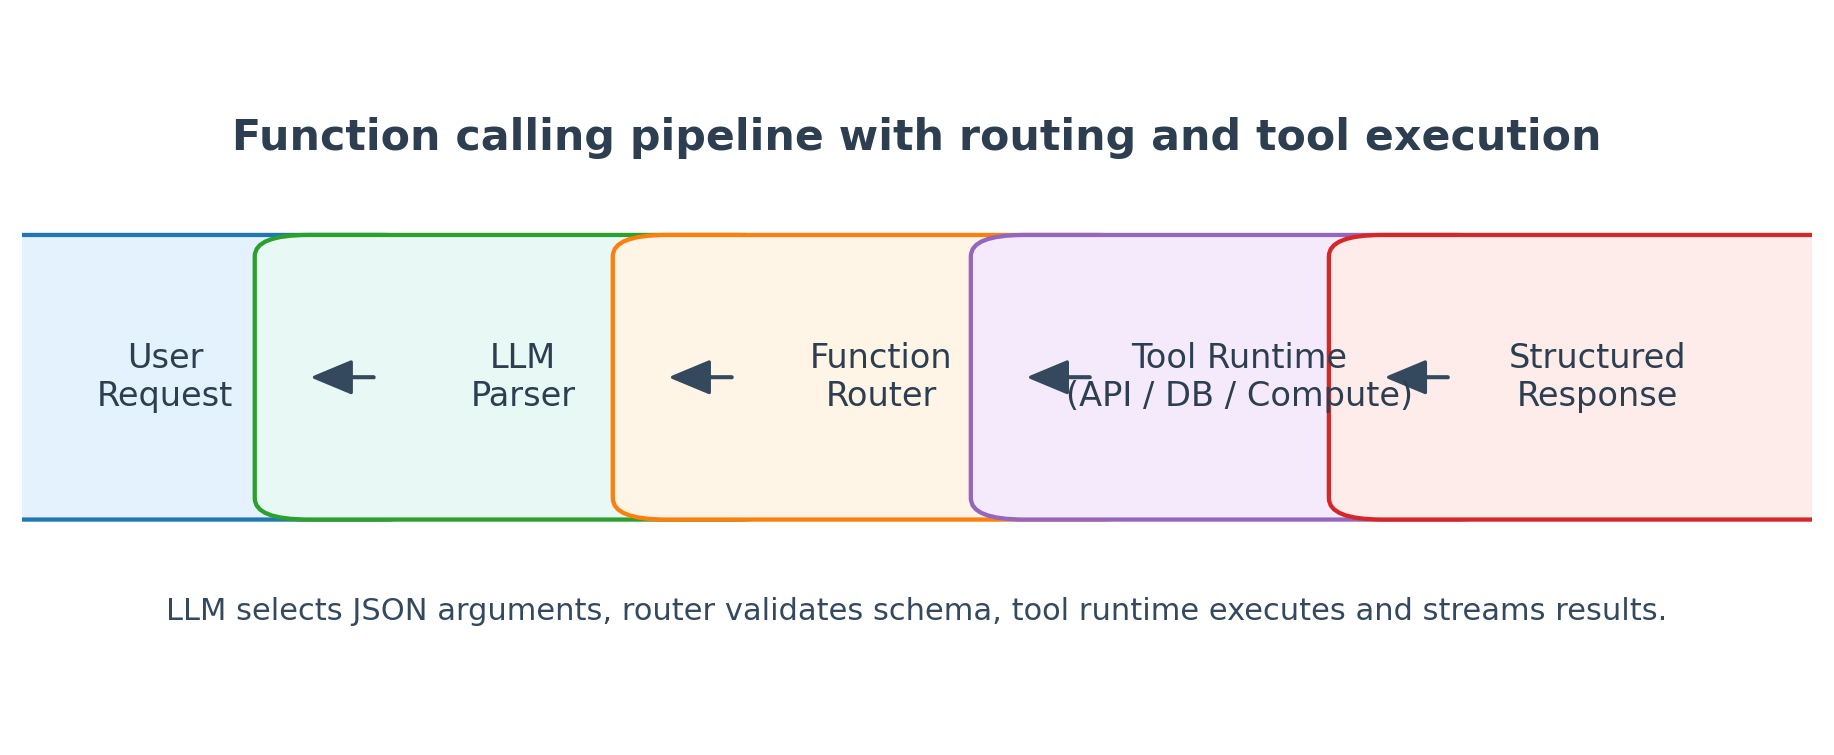
\includegraphics[width=0.9\textwidth]{function_calling_pipeline.png}
  \caption{函数调用流水线:解析、路由、工具执行与结构化响应。}
  \label{fig:function_pipeline_cn}
\end{figure}

\subsection{OpenAI 与 Anthropic 的实现差异}
\begin{longtable}{p{3.5cm}p{5cm}p{5cm}}
\toprule
维度 & OpenAI Function Calling & Anthropic Tool Use \\
\midrule
接口定义 & \texttt{functions} 字段,使用 JSON Schema 定义参数;支持多函数候选 & \texttt{tools} 字段,使用 \texttt{input\_schema} 指定 JSON Schema;可带 \texttt{cache\_control} \\
模型响应 & \texttt{tool\_calls} 数组,包含函数名与参数;可一次返回多个调用 & 消息流中嵌入 \texttt{tool\_use}/\texttt{tool\_result} 片段,保持流式输出 \\
自洽策略 & 模型可请求 \texttt{none} 表示直接回答;客户端决定是否继续循环 & Anthropic 建议“tool loop”:模型调用工具—等待结果—继续推理 \\
错误处理 & 客户端自行捕获异常并回传错误信息供模型重试 & 可通过 \texttt{tool\_result} 返回状态码、错误描述;模型可感知失败并修正 \\
安全控制 & 通过函数白名单、参数校验、代理层保护;支持 Rejection Sampling & 支持设置 \texttt{max\_tool\_outputs},并在 Prompt 中声明安全/合规策略 \\
\bottomrule
\end{longtable}

\subsection{函数调用代码示例}
\begin{lstlisting}[language=Python,caption={OpenAI 函数调用示例:调用天气 API}]
from openai import OpenAI
import requests

client = OpenAI(api_key="sk-...")

functions = [
    {
        "name": "get_weather",
        "description": "Retrieve weather data for a given city",
        "parameters": {
            "type": "object",
            "properties": {
                "city": {"type": "string"},
                "unit": {"type": "string", "enum": ["celsius", "fahrenheit"]}
            },
            "required": ["city"]
        },
    }
]

def call_weather(city: str, unit: str = "celsius") -> str:
    resp = requests.get("https://wttr.in", params={"format": "j1", "q": city})
    data = resp.json()
    temp = data["current_condition"][0]["temp_C" if unit == "celsius" else "temp_F"]
    return f"The temperature in {city} is {temp}°{unit[0].upper()}."

messages = [{"role": "user", "content": "What's the weather like in Reykjavik?"}]
response = client.chat.completions.create(
    model="gpt-4o-mini",
    messages=messages,
    functions=functions,
)

tool_call = response.choices[0].message.tool_calls[0]
args = tool_call.function.arguments
result = call_weather(args["city"], args.get("unit", "celsius"))

messages.extend([
    response.choices[0].message,
    {"role": "tool", "tool_call_id": tool_call.id, "name": "get_weather", "content": result},
])

final = client.chat.completions.create(model="gpt-4o-mini", messages=messages)
print(final.choices[0].message.content)
\end{lstlisting}

\section{ReAct + Tool + Memory 混合架构}
\subsection{框架组合}
混合架构将 ReAct(Reason + Act)链式推理、工具调用与记忆系统结合,实现持续对话与上下文感知。流程包括:
\begin{itemize}
  \item \textbf{思考(Thought):} 模型生成下一步策略,决定是否需要工具;
  \item \textbf{行动(Action):} 通过函数调用或插件执行操作;
  \item \textbf{观察(Observation):} 处理返回结果,更新记忆;
  \item \textbf{记忆写入:} 将关键信息存入短期对话记忆与长期向量记忆,支撑后续推理。
\end{itemize}

\subsection{记忆设计}
\begin{itemize}
  \item \textbf{短期记忆:} 存储最近对话与工具交互,便于模型保持语境;
  \item \textbf{长期记忆:} 通过向量数据库记录用户偏好、历史任务、重要事实;
  \item \textbf{工作记忆:} 任务执行过程中的临时变量、草稿、代码片段,任务完成后可清理或归档。
\end{itemize}

\subsection{安全与治理}
\begin{itemize}
  \item 对记忆写入实施过滤,避免敏感信息泄露;
  \item 使用 Guardrail 模型审核工具返回结果和模型下一步行动;
  \item 为不同工具设置频率限制与幂等校验,降低滥用风险。
\end{itemize}

\section{WebAgent / OS-Agent 实现思路}
\subsection{整体堆栈}
WebAgent 与 OS-Agent 通过不同的工具层与上下文缓存对接浏览器或操作系统。图\ref{fig:hybrid_agent_stack_cn} 展示了两类 Agent 与共享记忆、治理层的协同。
\begin{figure}[H]
  \centering
  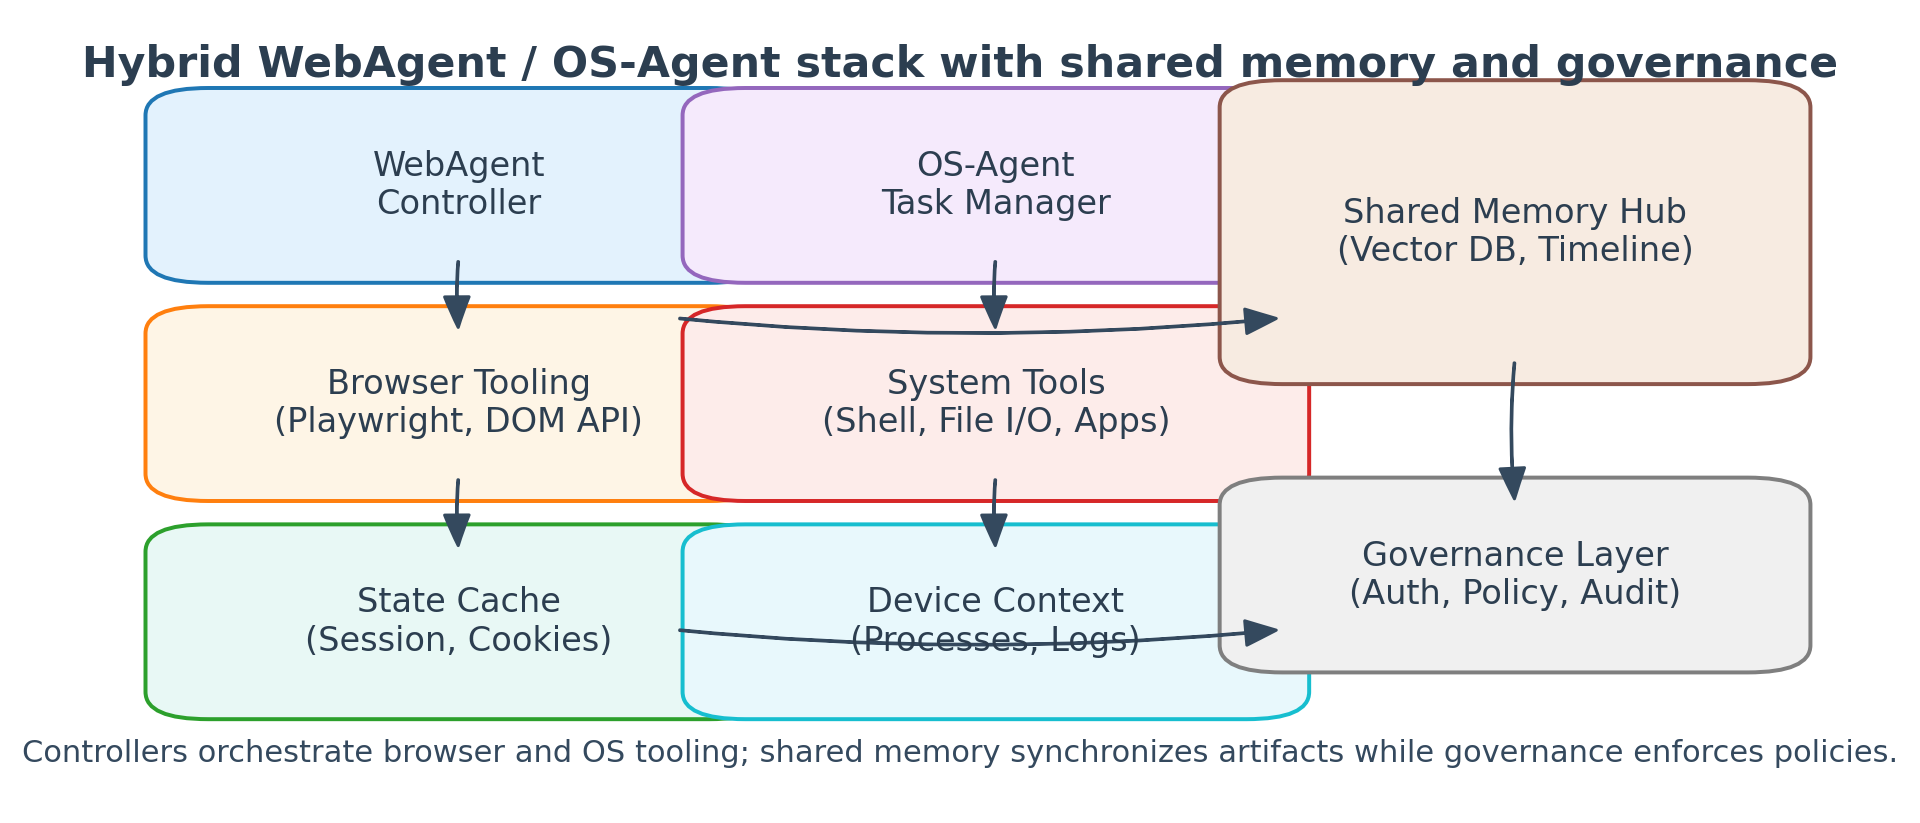
\includegraphics[width=0.9\textwidth]{hybrid_agent_stack.png}
  \caption{WebAgent / OS-Agent 混合堆栈:控制器、工具、状态缓存与治理层。}
  \label{fig:hybrid_agent_stack_cn}
\end{figure}

\subsection{WebAgent 关键组件}
\begin{itemize}
  \item \textbf{浏览器控制:} 基于 Playwright、Selenium、puppeteer 等驱动 DOM 交互;
  \item \textbf{页面理解:} 结合 HTML 解析、Vision-Language 模型、可视化快照,生成结构化描述;
  \item \textbf{状态管理:} 会话、Cookie、localStorage 缓存,支持跨页面任务;
  \item \textbf{安全防护:} 防止点击危险链接、执行脚本注入,通过策略引擎进行白名单校验。
\end{itemize}

\subsection{OS-Agent 关键组件}
\begin{itemize}
  \item \textbf{系统工具:} 终端命令、文件系统、应用程序 API、脚本解释器;
  \item \textbf{设备上下文:} 进程列表、日志、权限状态、网络连接;
  \item \textbf{任务管理:} 计划任务、进度追踪、回滚机制、异常捕获;
  \item \textbf{治理层:} 访问控制、凭证管理、操作审计,确保系统安全。
\end{itemize}

\subsection{共享记忆与协同}
WebAgent 与 OS-Agent 可通过共享向量缓存、事件时间线同步任务信息,支持跨平台协作(例如先在浏览器收集资料,再在本地整理报告)。

\section{外部 API 与插件系统集成}
\subsection{插件生态}
\begin{itemize}
  \item \textbf{API 插件:} 例如 Slack、GitHub、Jira、Salesforce,提供标准化 webhook 与 OAuth 授权;
  \item \textbf{数据插件:} 连接数据库、数据湖、知识图谱,提供查询与写入接口;
  \item \textbf{自定义插件:} 企业内部服务的封装,需要明确参数 schema、权限策略。
\end{itemize}

\subsection{集成模式}
\begin{itemize}
  \item \textbf{直接函数调用:} 在函数注册表中定义插件接口,由 LLM 直接选择执行;
  \item \textbf{代理层:} 使用中间服务对请求进行二次验证、重试和日志记录;
  \item \textbf{工作流编排:} 将插件调用纳入 BPMN / workflow 引擎,与人工审批节点结合。
\end{itemize}

\subsection{API 安全策略}
\begin{itemize}
  \item 使用 JWT/OAuth2 进行身份验证,设置短期令牌并定期轮换;
  \item 记录调用审计日志,识别异常峰值、重复失败尝试;
  \item 对响应内容进行过滤与脱敏,避免敏感信息写入记忆。
\end{itemize}

\subsection{插件调用示例}
\begin{lstlisting}[language=Python,caption={调用 Notion 数据库插件并写入结果}]
import requests
import os

NOTION_TOKEN = os.environ["NOTION_TOKEN"]
DATABASE_ID = os.environ["NOTION_DB"]

headers = {
    "Authorization": f"Bearer {NOTION_TOKEN}",
    "Notion-Version": "2022-06-28",
    "Content-Type": "application/json",
}

payload = {
    "parent": {"database_id": DATABASE_ID},
    "properties": {
        "Title": {"title": [{"text": {"content": "Geothermal Report"}}]},
        "Status": {"select": {"name": "In Progress"}},
    },
    "children": [
        {"object": "block", "type": "paragraph", "paragraph": {"rich_text": [
            {"type": "text", "text": {"content": "Initial findings added by tool agent."}}
        ]}}
    ],
}

resp = requests.post("https://api.notion.com/v1/pages", headers=headers, json=payload, timeout=15)
resp.raise_for_status()
\end{lstlisting}

\section*{实践建议}
\begin{itemize}
  \item 为函数调用和插件接口统一制定 JSON Schema,便于自动校验与文档化。
  \item 建立工具调用的回放系统,对异常操作进行可视化排查、回滚与再训练。
  \item 在混合架构中使用“人类在环”审批节点,确保关键操作受控执行。
  \item 定期执行安全红队测试,验证工具层和治理层对异常行为的拦截能力。
\end{itemize}

\section*{参考文献}
\begin{itemize}
  \item OpenAI. ``Function calling and other API updates.'' 2023.
  \item Anthropic. ``Tool Use Capabilities in Claude.'' Technical Note, 2024.
  \item Yao et al. ``ReAct: Synergizing Reasoning and Acting in Language Models.'' ICLR, 2023.
  \item Qin et al. ``WebArena: A Realistic Web Environment for Building Autonomous Agents.'' NeurIPS, 2023.
  \item Microsoft Research. ``TaskMatrix.AI: Empowering LLMs with OS-Level Tool Augmentation.'' arXiv, 2023.
\end{itemize}

\end{document}

